\lecture{2}{lun 01 mag 2023 17:06}{Libreria di sistemi elementari}
	\lablsection{Libreria di sistemi elementari}
	% --- Resistore ---
	\lablsubsection{Resistore}
	\begin{figure}[H]
		\begin{minipage}{.3\textwidth}
			\centering
			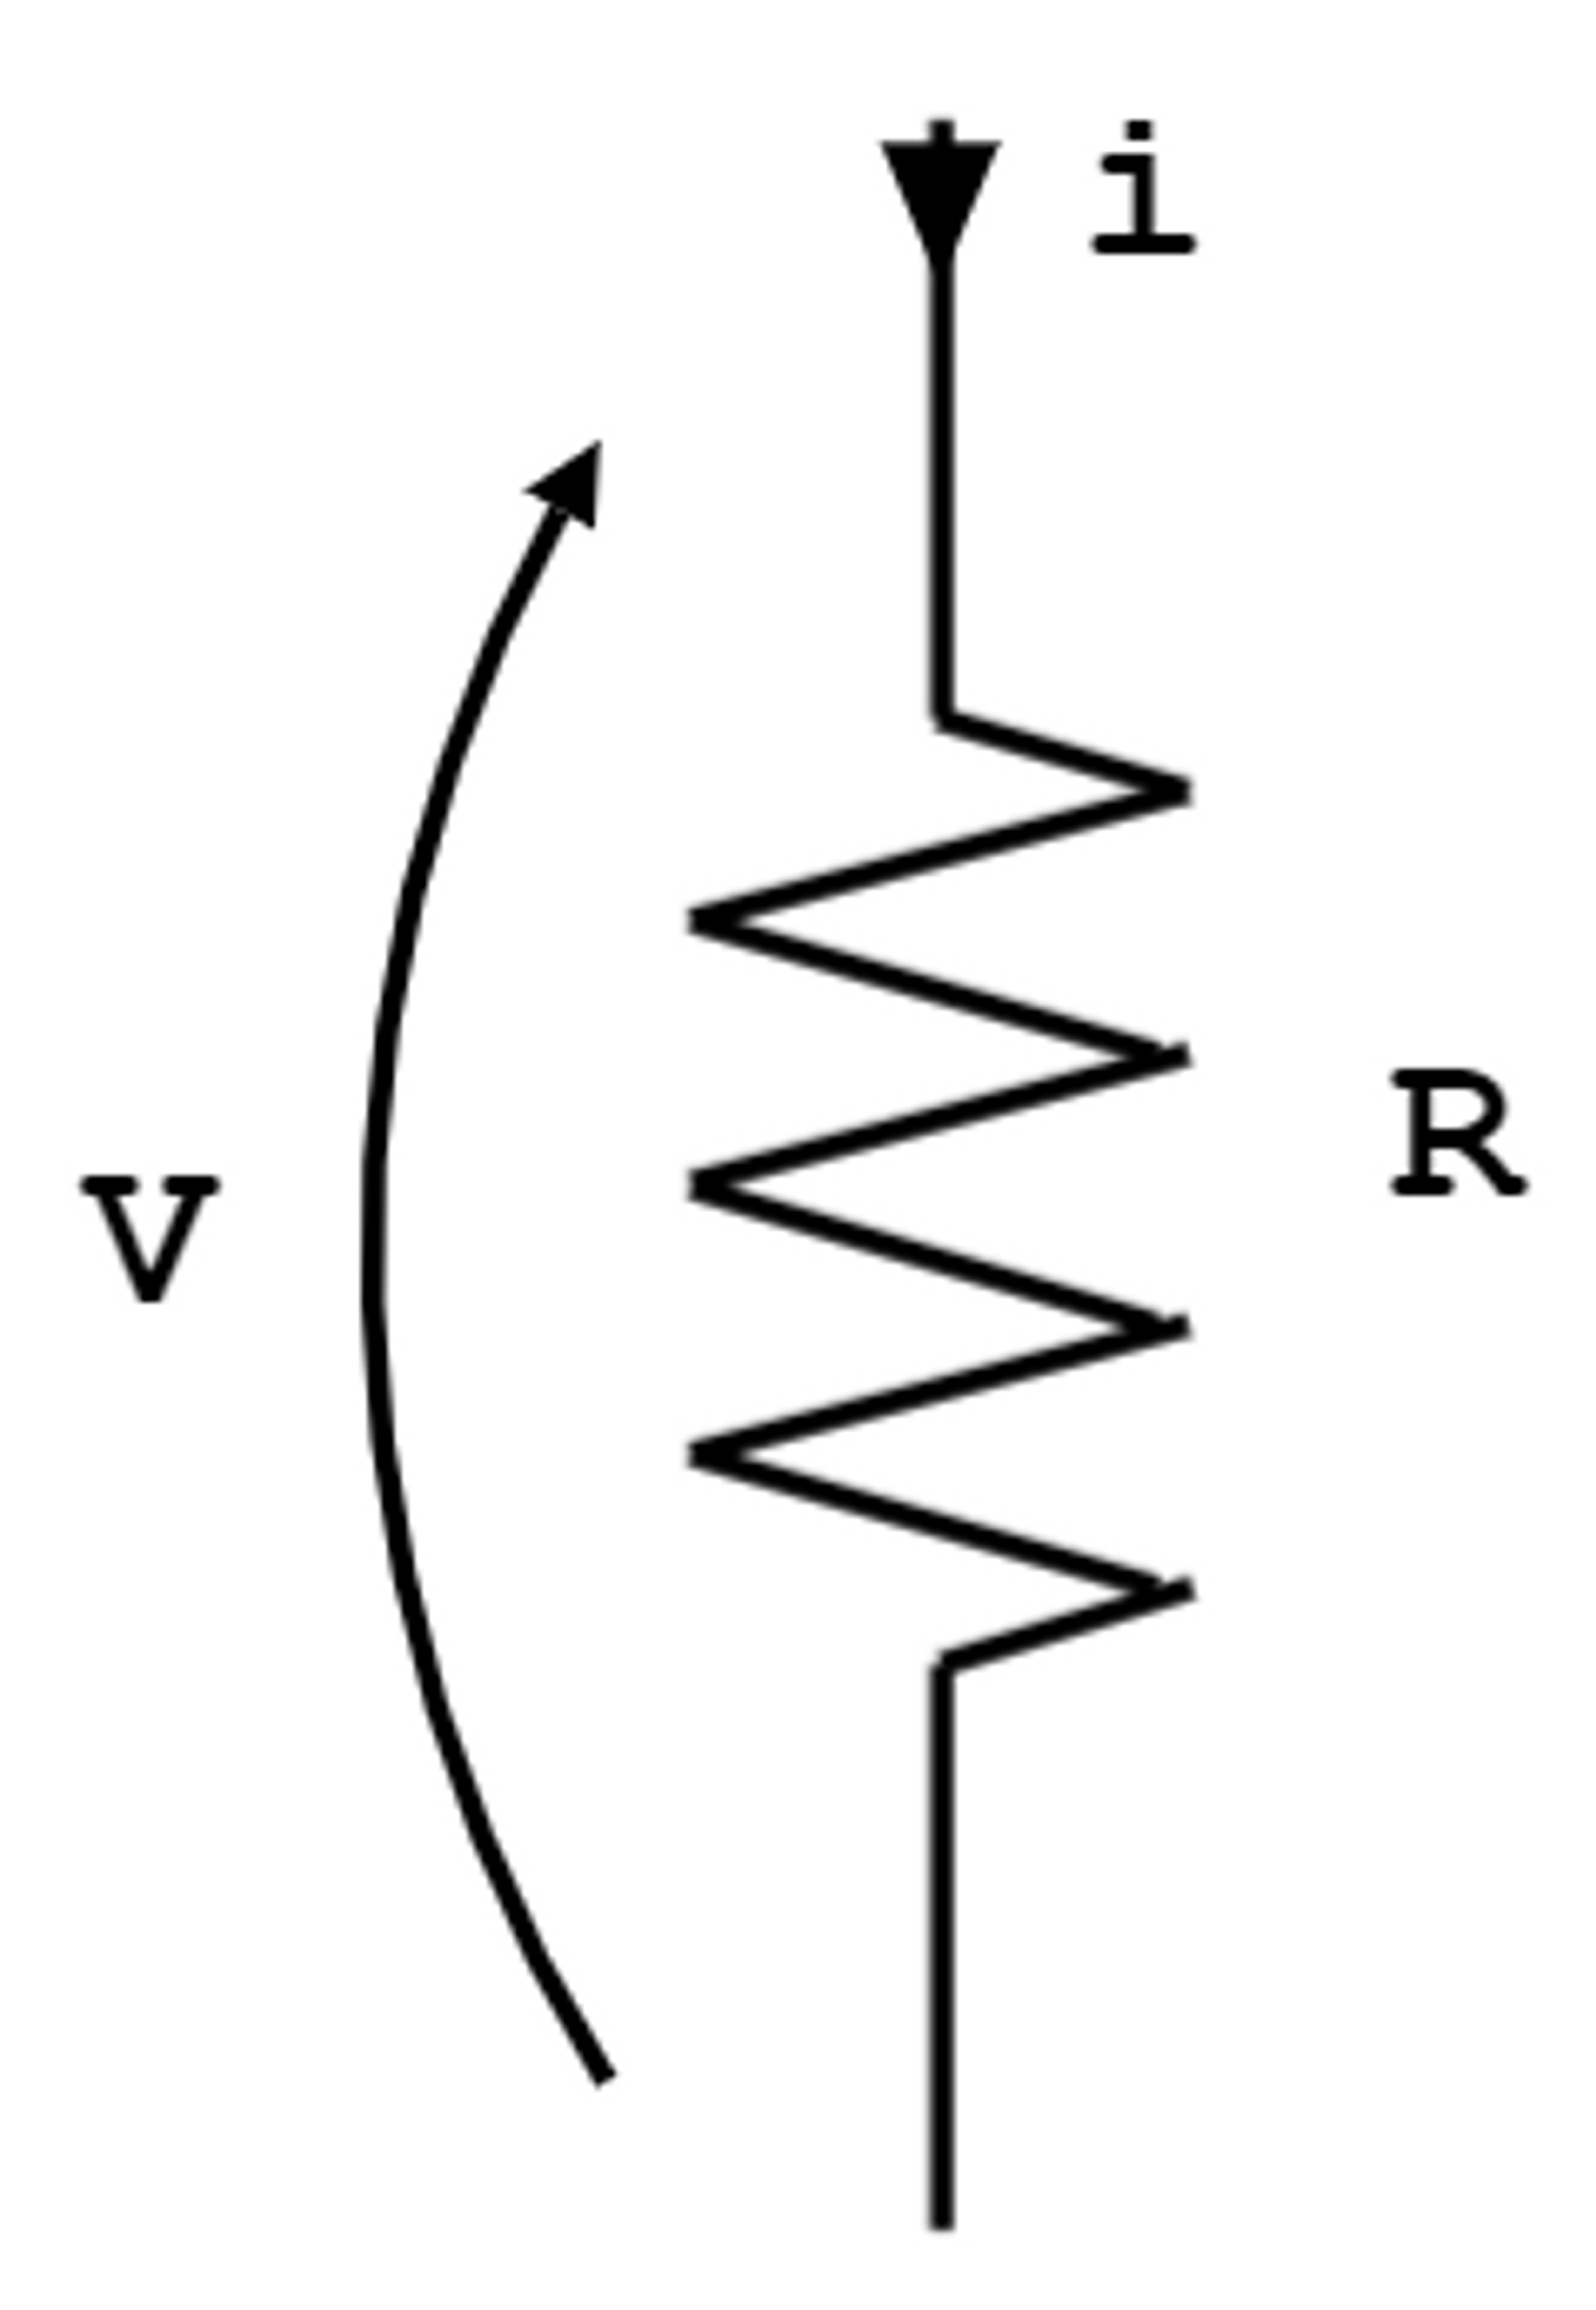
\includegraphics[width=.4\linewidth]{"Images/resistore.png"}
		\end{minipage}%
		\begin{minipage}{.3\textwidth}
			\begin{itemize}
				\item R: resistenza
				\item V: tensione
				\item i: corrente
			\end{itemize}
		\end{minipage}
		\begin{minipage}{.3\textwidth}
			\centering
			\begin{equation*}
				\boxed{\text{V} = \text{R}i}
			\end{equation*}
		\end{minipage}
	\end{figure}
	
	% --- Induttore ---
	\lablsubsection{Induttore}
	\begin{figure}[H]
		\begin{minipage}{.3\textwidth}
			\centering
			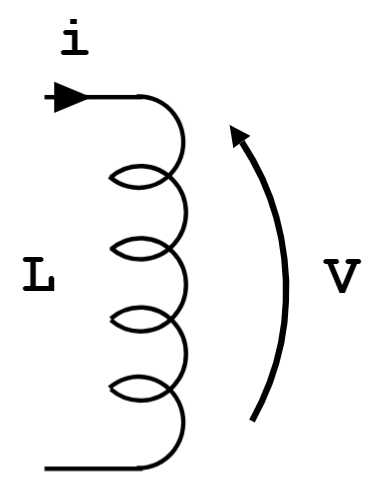
\includegraphics[width=.4\linewidth]{"Images/induttore.png"}
		\end{minipage}%
		\begin{minipage}{.3\textwidth}
			\begin{itemize}
				\item L: induttanza
				\item V: tensione
				\item i: corrente
			\end{itemize}
		\end{minipage}
		\begin{minipage}{.3\textwidth}
			\centering
			\begin{equation*}
				\boxed{\text{V} = \text{L}\frac{di}{dt} = \text{L} \dot{i}}
			\end{equation*}
		\end{minipage}
	\end{figure}
	
	% --- Condensatore ---
	\lablsubsection{Condensatore}
	\begin{figure}[H]
		\begin{minipage}{.3\textwidth}
			\centering
			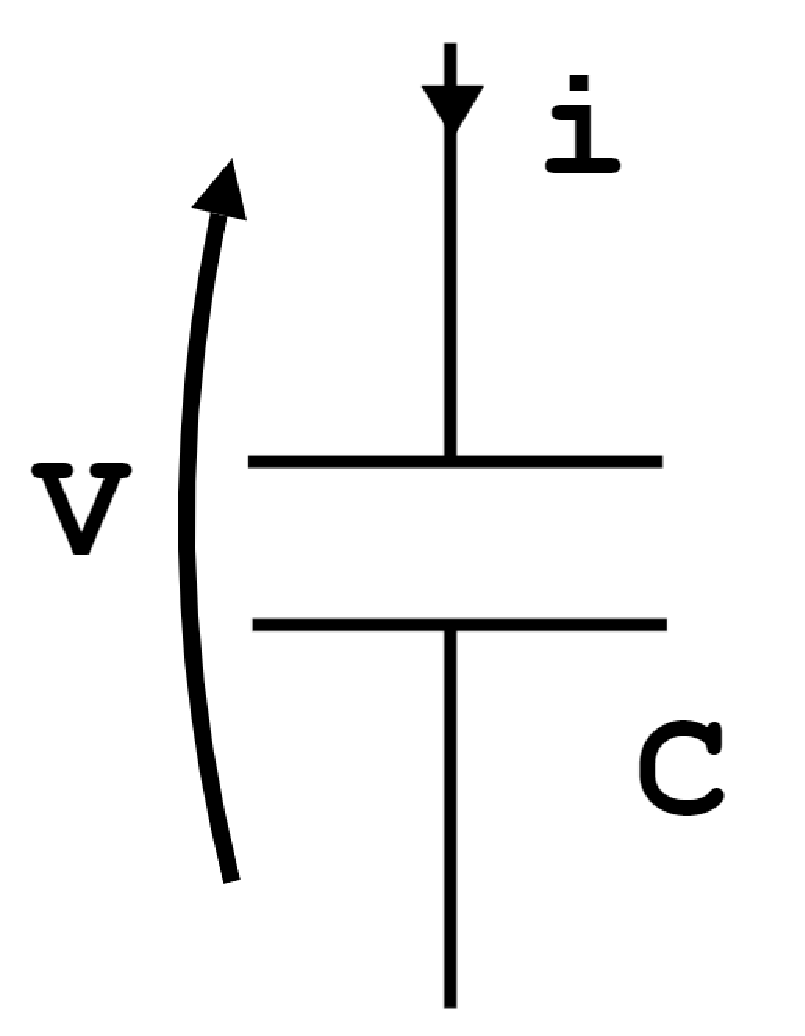
\includegraphics[width=.4\linewidth]{"Images/condensatore.png"}
		\end{minipage}%
		\begin{minipage}{.3\textwidth}
			\begin{itemize}
				\item C: capacità
				\item V: tensione
				\item i: corrente
			\end{itemize}
		\end{minipage}
		\begin{minipage}{.3\textwidth}
			\centering
			\begin{equation*}
				\boxed{\frac{d\text{V}}{dt} = \frac{1}{\text{C}}i}
			\end{equation*}
		\end{minipage}
	\end{figure}
	
	% --- Massa ---
	\lablsubsection{Massa}
	\begin{figure}[H]
		\begin{minipage}{.3\textwidth}
			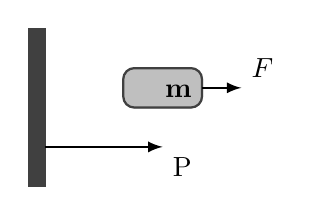
\begin{tikzpicture}[thick]
				\filldraw[color=darkgray] (-.2,0) rectangle (0,2);
				\draw[-latex] (0,.5) -- (1.5,.5)node[below right]{P};
				\filldraw[rounded corners,lightgray] (1,1.5) rectangle (2,1) node[above left,black]{$ \textbf{m} $};
				\draw[rounded corners,darkgray] (1,1.5) rectangle (2,1);
				\draw [-latex] (2,1.25) -- (2.5,1.25) node[above right]{$ F $};
			\end{tikzpicture}
			%			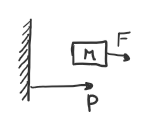
\includegraphics[width=.6\linewidth]{"Images/massa.png"}
		\end{minipage}%
		\begin{minipage}{.3\textwidth}
			\begin{itemize}
				\item M: massa
				\item P: posizione
				\item v: velocità
				\item a: accelerazione
				\item F: forza
			\end{itemize}
		\end{minipage}
		\begin{minipage}{.3\textwidth}
			\centering
			\begin{equation*}
				\boxed{F = ma}\text{  }
				\boxed{a = \frac{dv}{dt}}\text{  }
				\boxed{v = \frac{dP}{dt}}
			\end{equation*}
		\end{minipage}
	\end{figure}
	
	% --- Oscillatore Armonico ---
	\lablsubsection{Oscillatore armonico}
	\begin{figure}[H]
		\begin{minipage}{.3\textwidth}
			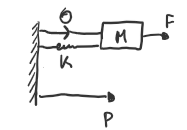
\includegraphics[width=.6\linewidth]{"Images/oscillatorearmonico.png"}
			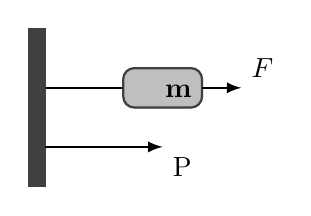
\begin{tikzpicture}[thick]
				\draw[decorate,decoration={coil,segment length=5pt,aspect=0.7,amplitude=4pt,pre=lineto,pre length=5mm,post=lineto,post length=5mm},thick] (0,1.25) -- (1,1.25);
				\filldraw[darkgray] (-.2,0) rectangle (0,2);
				\draw[-latex] (0,.5) -- (1.5,.5)node[below right]{P};
				\filldraw[rounded corners,lightgray] (1,1.5) rectangle (2,1) node[above left,black]{$ \textbf{m} $};
				\draw[rounded corners,darkgray] (1,1.5) rectangle (2,1);
				\draw [-latex] (2,1.25) -- (2.5,1.25) node[above right]{$ F $};
			\end{tikzpicture}
		\end{minipage}%
		\begin{minipage}{.3\textwidth}
			\begin{itemize}
				\item M: massa
				\item P: posizione
				\item v: velocità
				\item a: accelerazione
				\item F: forza
				\item K: costante elastica
				\item $ \sigma $: coefficiente di attrito
			\end{itemize}
		\end{minipage}
		\begin{minipage}{.3\textwidth}
			\centering
			\begin{equation*}
				\boxed{F = Kp + \sigma v + Ma}
			\end{equation*}
		\end{minipage}
	\end{figure}
	
	% --- Pendolo Semplice ---
	\lablsubsection{Pendolo semplice}
	\begin{figure}[H]
		\begin{minipage}{.3\textwidth}
			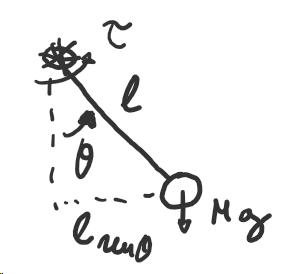
\includegraphics[width=.6\linewidth]{"Images/pendolosemplice.png"}
		\end{minipage}%
		\begin{minipage}{.3\textwidth}
			\begin{itemize}
				\item M: massa
				\item $ \tau $: coppia
				\item $ \theta $: posizione angolare
				\item $ \omega $: velocità angolare
				\item $ \alpha $:accelerazione angolare
				\item $ l $: lunghezza
				\item $ g $: accelerazione gravitazionale
			\end{itemize}
		\end{minipage}
		\begin{minipage}{.3\textwidth}
			\centering
			\begin{equation*}
				\boxed{\alpha = \frac{d\omega}{dt}}\text{ }
				\boxed{\omega = \frac{d\theta}{dt}}\text{  }
				\tau = \underbrace{Ml^2\alpha + Mgl\sin\theta}_{\textit{non lineare}}
			\end{equation*}
		\end{minipage}
	\end{figure}
	
	% --- Serbatoio Cilindrico ---
	\lablsubsection{Serbatoio cilindrico}
	\begin{figure}[H]
		\begin{minipage}{.3\textwidth}
			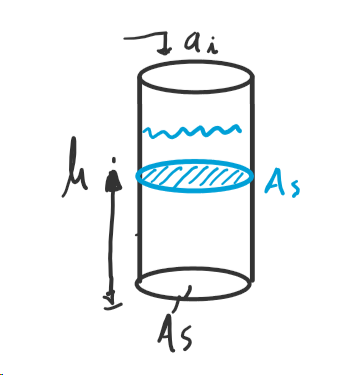
\includegraphics[width=.6\linewidth]{"Images/serbatoiocilindrico.png"}
		\end{minipage}%
		\begin{minipage}{.3\textwidth}
			\begin{itemize}
				\item $ A_s $: area sezione
				\item $ h $: livello liquido
				\item $ q_i $: portata ingresso
			\end{itemize}
		\end{minipage}
		\begin{minipage}{.3\textwidth}
			\centering
			\begin{equation*}
				\boxed{q_i = A_s \dfrac{dh}{di}}
			\end{equation*}
		\end{minipage}
	\end{figure}
	
	%--- Serbatoio con Valvola ---
	\lablsubsection{Serbatoio con valvola}
	\begin{figure}[H]
		\begin{minipage}{.3\textwidth}
			\centering
			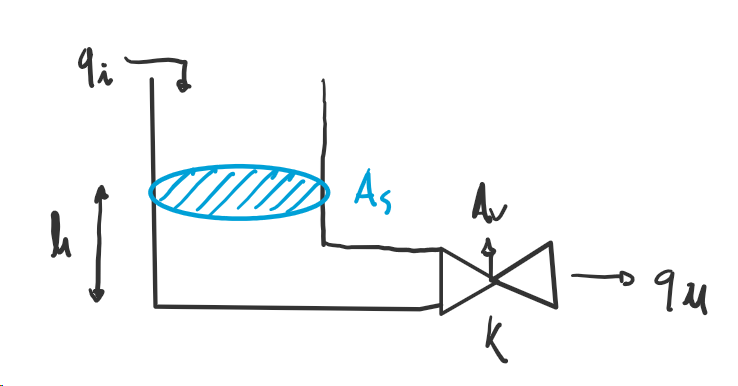
\includegraphics[width=0.9\linewidth]{"Images/serbatoioconvalvola.png"}
		\end{minipage}%
		\begin{minipage}{.3\textwidth}
			\begin{itemize}
				\item $ A_s $: area sezione
				\item $ h $: livello liquido
				\item $ q_i $: portata ingresso
				\item $ A_v $: area valvola
				\item $ k $: costante della valvola
			\end{itemize}
		\end{minipage}
		\begin{minipage}{.3\textwidth}
			\centering
			\begin{equation*}
				\boxed{q_u = \frac{dh}{dt}A_s}\text{  }q_i = \underbrace{A_s \dfrac{dh}{di} + k A_v \sqrt{h}}_{\textit{non lineare}}
			\end{equation*}
		\end{minipage}
	\end{figure}
%%% Local Variables:
%%% mode: latex
%%% TeX-master: "master"
%%% End:
